%!TEX root = ../report.tex

\chapter{Stereovision} % (fold)
\label{chap:stereopsis}

\section{Introduction}
In this section, the solution adopted for the location of the target in the 3D space through the vision system, the reasons that led to this approach, the assumptions made and the obtained results are presented.
A more detailed explanation of the 2D image processing performed for the target tracking can be found in \ref{chap:feature_extraction}.

\section{Stereopsis}
Due to the fact that two vision systems were available on the setup, the first step was to decide which one to employ and the method to compute disparity.
After a slight evaluation of resources the chosen one was the stereo rig, utilized to carry out sparse stereo with a single well-defined point.
Thus, the next points contain the steps to compute the position of a point in 3-space given its image in two views and the camera matrices.

Through the acquired pairs of images, the pixel coordinates of the center of gravity of the target are extracted by the algorithm presented in \ref{chap:feature_extraction}.
They are used to calculate its 3D coordinates referred to the camera reference frame by means of linear triangulation methods.

\section{Camera model}
As a consequence of the need of a defined relation between the image and the object space, the cameras must be used as a mapping.
The mathematical model assumed for the camera is the basic pinhole structure, described in \cite{Hartley}.
This model defines a linear projection from the 3D world to the image plane, and contains the intrinsic parameters that relates the camera and the image reference frames as showed in equation \eqref{eq:pinhole_model}. Where X represent the homogeneous coordinates of a 3D point and x its projection in the image plane in pixel coordinates.

\begin{equation}
x = P \cdot X
\label{eq:pinhole_model}
\end{equation}

Since the linearity assumed by this model does not hold due to imperfections in the lens, a distortion model needs to be added to the calculations in order to correct the deviations on the real cameras.
The Plumb Bob distortion model, introduced in \cite{Brown} is applied here since it is the one used by ROS.

\subsection{Camera calibration}
\label{sec:cam_calib}
In order to obtain the intrinsic parameters for the camera model, a stereo calibration process based on a 2D pattern has been carried out for both Bumblebee2 1394a cameras by means of a ROS node. The procedure and some basics of it are to be found in \ref{sec:camera_calibration}.

\section{3D Reconstruction}
In order to compute the depth for a pair of correspondent image points, a suitable triangulation method light but robust enough to be executed on line with sufficient accuracy must be found.
The task, trivial in theory, entails certain complexity due to the acquisition errors in the measured image coordinates.
An immediate, simple approach could consists in back-projecting the correspondent image points, by means of the projection matrices, and finding the 3D point in the space in which they intersect.
However, this procedure is very unlikely to succeed in most of the cases since the image points do not satisfy the epipolar constraint due the errors.

\begin{figure}[h]
    \centering
    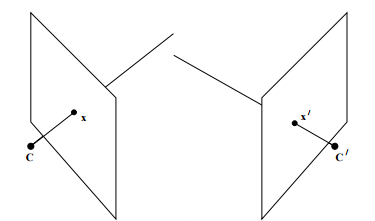
\includegraphics[width=0.8\textwidth]{figures/back_projection}
    \caption{Back-Projection rays error}
    \label{fig:Back-Projection}
\end{figure}

This is because in most of the cases the rays will not intersect in the 3D point, since there is not a point X that satisfies the equations \eqref{eq:projection}.

\begin{align}
\begin{split}
	x  &= P X\\
	x' &= P' X
	\label{eq:projection}
\end{split}
\end{align}

\subsection{Triangulation}
The applied method to estimate depth and compute the estimations of 3D positions is the defined for the OpenCV functions utilized in the developed algorithm.
This method is based on the direct linear transformation procedure to compute the estimation of the 3D point.

\subsubsection{Direct Linear Transformation}
The equations \eqref{eq:projection} are combined into a set of linear equations in X of the form \eqref{eq:DLT} by eliminating the scale factor, where the matrix A is \eqref{eq:DLT2}

\begin{equation}
	AX = 0
	\label{eq:DLT}
\end{equation}

\begin{equation}
A =
 \begin{pmatrix}
  xP^{3T} - P^{1T} \\
  yP^{3T} - P^{2T} \\
  x'P^{'3T} - P^{'1T} \\
  yP^{'3T} - P^{'2T}
 \end{pmatrix}
 \label{eq:DLT2}
\end{equation}

The way the DTL algorithm solves this set of redundant equations in the unknowns of X is by means of a Least-squares minimization problem in the absence of an exact solution.
The presence of noise reduces the problem to the minimization of \eqref{eq:LSM} where e stands for the projection errors.
The LS solution solution is given in equation \eqref{eq:LSM_solution}.

\begin{equation}
	\centering
	\lVert \mathbf{AX-e} \rVert
	\label{eq:LSM}
\end{equation}

\begin{equation}
	\centering
	X = [A^{T}A]^{-1}A^{T}e
	\label{eq:LSM_solution}
\end{equation}

It is known that a minimization of the geometric error for a given correspondent pair of points $\{x, x_i\}$.
The way to do so would be to minimize the sum of squared distances to find a pair of points $\{\hat{x}, \hat{x}_i\}$ subject to the epipolar constraint.
However, not enough documentation about OpenCV was found in order to find out if this process is implemented in the applied functions.

\section{Experiments}
Under this section the approach to the experimentation and the final results obtained are to be found.
The tests for the overall performance of the triangulation algorithm, together with the 2D detector have been carried out once the robotics part was operative.
Thus, it has been possible to test the on line triangulation through the analysis of the movement of the robot in relation to the target.
The idea was to check manually if the triangulation was able to keep the camera pointing to the target and at the specified distance once the path planner was tested and working.



% section stereopsis (end)

